\documentclass[11pt]{article}

\usepackage[utf8]{inputenc}
\usepackage{fancyhdr}
\usepackage{hyperref}
\usepackage{graphicx}

\graphicspath{ {images/} }
 
\pagestyle{fancy}
\fancyhf{}
\lhead{University of the Witwatersrand}
\rfoot{School of Computer Science and Applied Mathematics}
\pagenumbering{roman}
\fancyfoot[R]{\thepage}

\begin{document}
\begin{page}

\newcommand{\HRule}{\rule{\linewidth}{0.3mm}} % Defines a new command for the horizontal lines, change thickness here
\renewcommand\section{\@startsection{section}{1}{\z@}%
                                  {-3.5ex \@plus -1ex \@minus -.2ex}%
                                  {2.3ex \@plus.2ex}%
                                  {\normalfont\large\bfseries}}
\setlength{\parindent}{0pt}

\center % Center everything on the page
 
%----------------------------------------------------------------------------------------
% HEADING SECTIONS
%----------------------------------------------------------------------------------------

\textsc{\LARGE University of the Witwatersrand}\\[1.5cm] % Name of your university/college
\textsc{\Large School of Computer Science and Applied Mathematics}\\[0.5cm] % Major heading such as course name

%----------------------------------------------------------------------------------------
% TITLE SECTION
%----------------------------------------------------------------------------------------

\HRule \\[0.4cm]
{ \huge \bfseries COMS3008: Parallel Computing Lab Assignment 2}\\[0.4cm] % Title of your document \\
  \large 25 July 2016
\HRule \\[1.5cm]
 
%----------------------------------------------------------------------------------------
% AUTHOR SECTION
%----------------------------------------------------------------------------------------
\begin{minipage}{1\textwidth}
  \Large \emph By Chalom, J. (711985)\\
\end{minipage}


\vfill % Fill the rest of the page with whitespace

\end{page}

\begin{page}

\clearpage
\setcounter{page}{1}
\pagenumbering{arabic}

\section{General Assumptions and Methodology}
The computer which the decomposition of the factorial algorithm is to be run on only has two other processing units. This is a hybrid system which has both private memory spaces and shared memory spaces. The factorial algorithm being investigated will have the number 1 as the last number multiplied to the running variable in order to find the factorial as some integer $n$.\\

\noindent All drawn diagrams were drawn using \url{http://draw.io/}, and all results from empirical analysis, were statistically analysed by the data processing program used in lab 1. Those averaged results were then plotted using Microsoft Excel.\\

\noindent The system used for empirical analysis, had an i3 Ivy-bridge CPU, with four processing units and 8GB of RAM.

\section{Directed Acyclic Graphs}
\noindent \chapter{Chosen Decomposition:} \\
\noindent Let $n$ be the number whose factorial is being investigated. \\
$ n = \{ n \in \mathbb{Z}\ |\ 1 \leq n \leq \mathbb{Z}\} $ 
\\\\
\noindent \chapter{Data dependency of the chosen decomposition} \\
\begin{figure}[ht]
\centering
     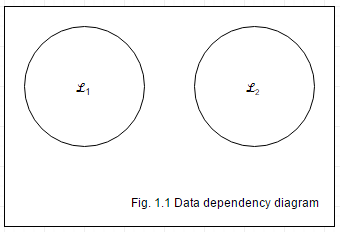
\includegraphics[width=0.80\textwidth]{parallel_fig_1_1}
\end{figure}

\noindent Let $L$ be the set of numbers constructed from n such that $L = \{ L \in \mathbb{Z}\ |\ n \leq L \leq 1\}$.
Therefore let $L_1$ and $L_2$ be subsets of $L$ such that $L \in (L_1 + L_2) $.

\noindent Let $i \in \mathbb{Z} \ s.t. \ 0 < i < n$.
Therefore $L_1 \in \{ n\ |\ (n - i)\ mod \ 2 = 0 \}$ and $L_2 \in \{ n\ |\ [(n - i) - 1]\ mod \ 2 = 0 \}$.\\
\noindent i.e. $L_1$ contains even numbers and $L_2$ contains odd numbers (up to n).\\

\noindent Figures 1.2.1 and 1.2.2 shows this decomposition of the data for the factorial algorithm.\\

\begin{figure}[ht]
\centering
     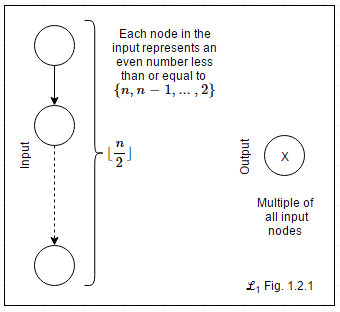
\includegraphics[width=0.80\textwidth]{parallel_fig_1_2_1}
\end{figure}

\begin{figure}[ht]
\centering
     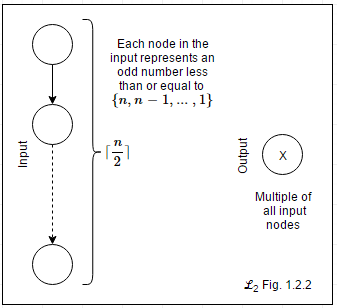
\includegraphics[width=0.80\textwidth]{parallel_fig_1_2_2}
\end{figure}\\

\break

\noindent \chapter{Task interaction of the chosen decomposition} \\

\noindent Let $T_1$, $T_2$ and $T_3$ be the tasks which make up the decomposition of the factorial operation.\\

\begin{figure}[ht]
\centering
     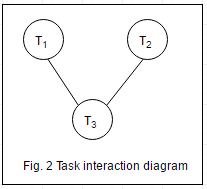
\includegraphics[scale=1]{parallel_fig_2}
\end{figure}
\\

\noindent $T_1$ uses the data-set $L_1$.\\
\noindent $T_2$ uses the data-set $L_2$.\\
\noindent $T_3$ uses the data-set $L_3$.\\

\noindent $T_1$ (even) and $T_2$ (Odd) both iterate through their respective data-sets and multiply a running variable by the next number in the data-set.
This variable is initialised by 1 and it becomes the answer of the previous iteration. \\
\noindent $T_3$ is the task which multiplies the respective results of $T_1$ and $T_2$.\\

\break
\noindent \chapter{Task dependency of the chosen decomposition} \\

\begin{figure}[ht]
\centering
     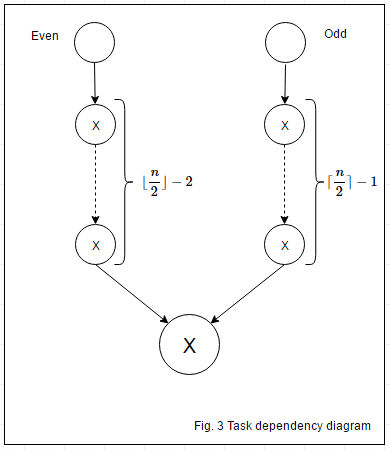
\includegraphics[scale=1]{parallel_fig_3}
\end{figure} \\

\noindent $T_1$ (even) and $T_2$ (Odd) lead to a barrier, which is $T_3$. This operation waits for both $T_1$ and $T_2$ to complete and then a reduction operation occurs - denoted here by: $X$. $T_3$ takes the results of $T_1$ and $T_2$ and multiplies them together to get the final result, which means that both $T_1$ and $T_2$ have to complete before $T_3$ can be executed.\\

\noindent In this case both $T_1$ and $T_2$ have been denoted in fig 3 by their internal parts - the iterations which occur inside them. \\

\noindent If $n$ is odd then the number of nodes in $T_1$ is $\lfloor{\frac{n}{2}}\rfloor - 2$ and $T_2$ is $\lceil{\frac{n}{2}}\rceil - 1$. If $n$ is even then the number of nodes is reversed - where $T_2$ has the floor function applied. One task is left out and that is $T_3$. The other negative one is there to denote that odd numbers end in one. Anything that is multiplied by one stays the same, this fact helps to make sure that the number of operations at the end is always $n$, since an odd numbered $n$ will lead to a disparity between the size of $L_1$ and $L_2$.

\break

\section{Algorithm Complexity}
Assumptions made regarding the 
\noindent \chapter{Sequential Complexity:} \\
The complexity of the sequential algorithm is: $\ominus(n)$, where $n$ is the number being investigated as that many operations have to be completed to find the factorial.\\

\noindent \chapter{Recursive Complexity:} \\
The complexity of the recursive algorithm is: $\ominus(n + k)$, where $n$ is the number being investigated as that many operations have to be completed to find the factorial. $k$ is the arbitrary constant which represents the cost of the function recursively spawning itself $n$ times.\\

\noindent \chapter{Parallel Sequential Complexity:} \\
The internal time complexity of the sequential algorithm when it is parallelised is: $\ominus(log(\lfloor{\frac{n}{2}}\rfloor) + 1)$, where n is the number being investigated and 1 is the assumption that the reduction operator and final result takes constant time to complete. Another assumption that made is that both $T_1$ and $T_2$ complete their operations at roughly the same amount of time due to them having approximately the same number of operations to complete. The reason why this implementation is logarithmic in nature is because the implementation of a parallelised for loop in openMP will produce a parallelised reduction decomposition which is logarithmic.\\

\noindent The computational complexity of this decomposition is: $\ominus(n + k)$, where $n$ is the number being investigated as that many operations have to be completed to find the factorial and $k$ is a constant that represents the complexity of the reduction operator and the complexity of the final operation. This is because the parallel version can complete its calculation faster than the standard iterative approach but it cannot make the amount of computations required to complete the calculations any less.\\

\noindent \chapter{Parallel Recursive Complexity:} \\
The time complexity of a decomposition of the recursive algorithm is: $\ominus(\frac{n}{2} + k)$, where $n$ is the number being investigated and $k$ is a constant that represents the time taken due the reduction operations, wait factor of the different sections used and the time taken in memory due to executing the recursive operations of the algorithm. The algorithm is split into two sections which are computed in parallel which is why the time complexity is halved.\\

\noindent The computational complexity of this decomposition is: $\ominus(n + k)$, where $n$ is the number being investigated as that many operations have to be completed to find the factorial and $k$ is a constant that represents the complexity of the reduction operator and the internal recursive nature of each section. This is because the parallel version can complete its calculation faster than the standard recursive approach but it cannot make the amount of computations required to complete the calculations any less.\\ 

\break

\section{OpenMP Implementation}
\noindent The empirical analysis of each of the four algorithms was done by setting n to 1000 and running each algorithm 25 times, and then n is incremented by 1000. This process is repeated 500 times, to get results for n = 1000 to n = 500000.\\

\noindent Unfortunately algorithm 2, the sequential recursive algorithm has a stack limit of n = 261000, after which there is a segmentation fault. This is shown in the scatter plot (below) where algorithm 2 is just over half the amount of $n$ values tested than other three plots.\\

\noindent The total execution times of the algorithms (excluding algorithm 2) from n = 1000 to n = 500000 were also recorded.

\begin{table}[ht]
\centering
\begin{tabular}{|c|c|c|}
\hline
Algorithm 1 & Algorithm 3 & Algorithm 4 \\ \hline
\multicolumn{1}{|r|}{12.025520} & \multicolumn{1}{r|}{4.927197} & \multicolumn{1}{r|}{19.324828} \\ \hline
\end{tabular}
\caption{Completion Times Of Algorithms (in Seconds)}
\end{table}

\noindent From the table above you can see that the third algorithm (The parallel iterative algorithm is the fastest completing every calculation of the other algorithms tested.

\begin{figure}[ht]
\centering
     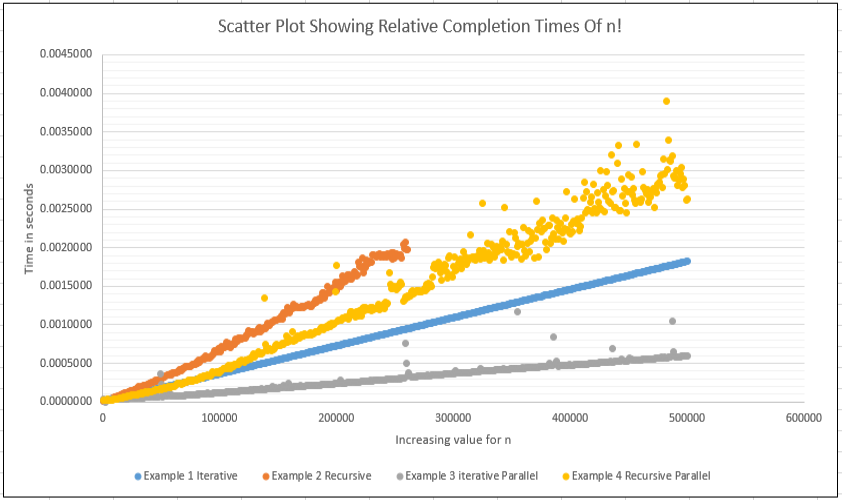
\includegraphics[scale=0.50]{scatter_plot}
\end{figure}\\

\noindent The scatter plot concurs with the execution times table because it shows the third algorithm being the fastest of the four. Another interesting observation is that the first algorithm which is the sequential iterative approach is the most predictable and 'stable' of the algorithms. Algorithm 2 seems to be the worst performing, and Algorithm 4 seems to be the most varied with data-points scattered the furthest from a line of best fit.\\

\noindent Algorithm 3's result can be explained by internal optimisations in openMP, specifically openMP parallelising the reduction operation - producing a tree decomposition of the algorithm.

\end{page}
\end{document}
